\documentclass[11 pt]{article}

\setlength{\oddsidemargin}{-.45in}
%\setlength{\evensidemargin}{-.5in}
\setlength{\textwidth}{7.25in}
\setlength{\topmargin}{-0.95in}
\setlength{\textheight}{10.2in}

\usepackage{graphics}
\usepackage{latexsym}
\usepackage{amsfonts}
\usepackage{amsmath}
\usepackage{amsthm}
\usepackage{epstopdf}
%\usepackage{multicol}
%\usepackage{wrapfig}
\pagestyle{empty}

\usepackage[T1]{fontenc}
\usepackage{baskervald}
\usepackage[bigdelims,vvarbb]{newtxmath} 

\newcommand{\ds}{\ensuremath{\displaystyle}}
\newcommand{\tr}{\vspace{0.5in}}
\newcommand{\lr}{\vspace{1.0in}}
\newcommand{\mr}{\vspace{2.0in}}
\newcommand{\br}{\vspace{3.0in}}

\newcommand{\ps}{Problem Set~}
\newcommand{\vi}{\ensuremath{\mathbf{i}}}
\newcommand{\vj}{\ensuremath{\mathbf{j}}}
\newcommand{\vk}{\ensuremath{\mathbf{k}}}
\newcommand{\vr}{\ensuremath{\mathbf{r}}}
\newcommand{\vecv}{\ensuremath{\mathbf{v}}}
\newcommand{\vu}{\ensuremath{\mathbf{u}}}
\newcommand{\va}{\ensuremath{\mathbf{a}}}
\newcommand{\vs}{\ensuremath{\mathbf{s}}}
\newcommand{\ve}{\ensuremath{\mathbf{e}}}
\newcommand{\vx}{\ensuremath{\mathbf{x}}}
\newcommand{\vc}{\ensuremath{\mathbf{c}}}
\newcommand{\vb}{\ensuremath{\mathbf{b}}}

\usepackage{hyperref} 
\hypersetup{colorlinks=true, linkcolor=blue,  anchorcolor=blue,  
citecolor=blue, filecolor=blue, menucolor=blue, pagecolor=blue,  
urlcolor=blue,pdftitle={MTH 202 Checkpoint}}

\usepackage{framed}

\newcommand{\bdr}{\ensuremath{\mathbb{R}}}

\newcommand{\be}{\begin{enumerate}}
\newcommand{\ee}{\end{enumerate}}

\newcommand{\bi}{\begin{itemize}}  
\newcommand{\ei}{\end{itemize}}

%\renewcommand{\baselinestretch}{1.5}


\begin{document}
 \hfill Boelkins \\
 
\begin{center}
Math 202-06 \\
{\bf Checkpoint 3}
\end{center}


\noindent {\bf Directions:}

\begin{itemize}
	
	\item {\bf Desmos.} You may use \href{https://www.desmos.com/calculator}{\emph{Desmos}} for computations and graphing, just like we do during class.  Any work done in \emph{Desmos} must be summarized and briefly explained in writing on your paper.  
	
	\item {\bf Resources.} During each checkpoint, you may access your own 1 page of study notes, plus \emph{Desmos}; no other uses of your computer or tablet are permitted unless specified directly.  No collaboration with other human beings or other internet resources are allowed.
	
%	\emph{Note well: if you collaborate with someone else, it is often obvious that collaboration has occurred.  Please do not put your academic standing at risk by doing this.}
	
	\item {\bf Competence.} Each week, your goal is to demonstrate competence on as many of the included learning targets as you can.  Each question will be marked either ``Y'' or ``NY'': Y for ``yes'', NY for ``not yet''.  Every learning target will appear on three different checkpoints, so you'll have multiple attempts to demonstrate your understanding.  ``Competence'' is defined as work that demonstrates clear and complete understanding of the relevant concepts in the learning target. While the work may include a minor error, or one or two minor steps may not be well explained, otherwise the work is complete, correct, and convincing, including the proper use of notation, and appropriate explanation of meaning that uses correct terminology.  (On rare occasions, you might get a ``NY*''; such a mark means you are close to competence and that you have the option to have a short conversation with me prior to the next Checkpoint and attempt to demonstrate ``Y''-level understanding through the conversation aloud.)	
\end{itemize}

\noindent \hrulefill \\

\noindent {\bf Learning Targets:} For Checkpoint \#3, there are four learning targets being assessed: 

\begin{quote}
{\bf LT 1}: I can do three key things from first semester calculus: (a) sketch the derivative function, given a function’s graph; (b) apply the chain rule to find the derivative of a composite function; and (c) apply the First Fundamental Theorem of Calculus to evaluate a definite integral. (Sections 1.4, 2.5, and 4.4)
\end{quote}

\begin{quote}
{\bf LT 2}: Given the graph of a function and other data, I can construct an accurate graph of the antiderivative of the function by determining select values of the antiderivative as well as where the antiderivative is increasing/decreasing and CCU/CCD.
(Section 5.1)
\end{quote}

\begin{quote}
{\bf LT 3}: I can apply the Second Fundamental Theorem of Calculus to find the antiderivative of a function in terms of an integral and also use the Second FTC to differentiate an integral function. (Section 5.2)
\end{quote}


\begin{quote}
{\bf LT 4}: I can use integration by substitution and integration by parts to evaluate integrals. (Sections 5.3-5.4)
\end{quote}

\noindent \hrulefill \\

\vfill \hfill {\bf OVER} 

\pagebreak

\noindent Name: \\ \ \\

\noindent To demonstrate competence on Learning Target \#n, you need to correctly respond to all or nearly all of the prompts in question \#n.  

\begin{enumerate}

%%% These are all the CP1 questions %%%

	\item[1.] 
	\be
		\item  For the function $f$ plotted at left, sketch an accurate graph of its derivative, $f'$, on the axes at right. \\  

\begin{center}  
  \scalebox{0.3}{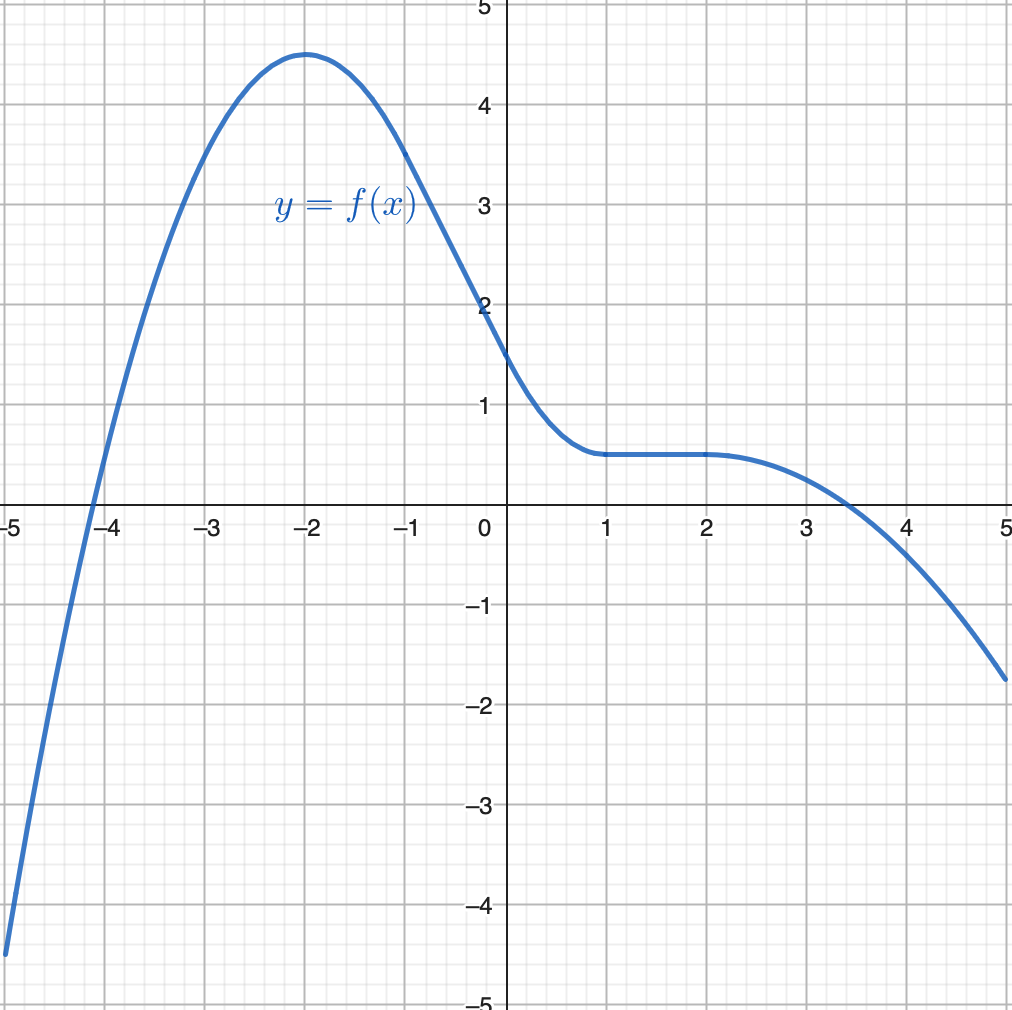
\includegraphics{images/CP-3-LT-1-graph-F23.png}} \hspace{0.25in} \scalebox{0.3}{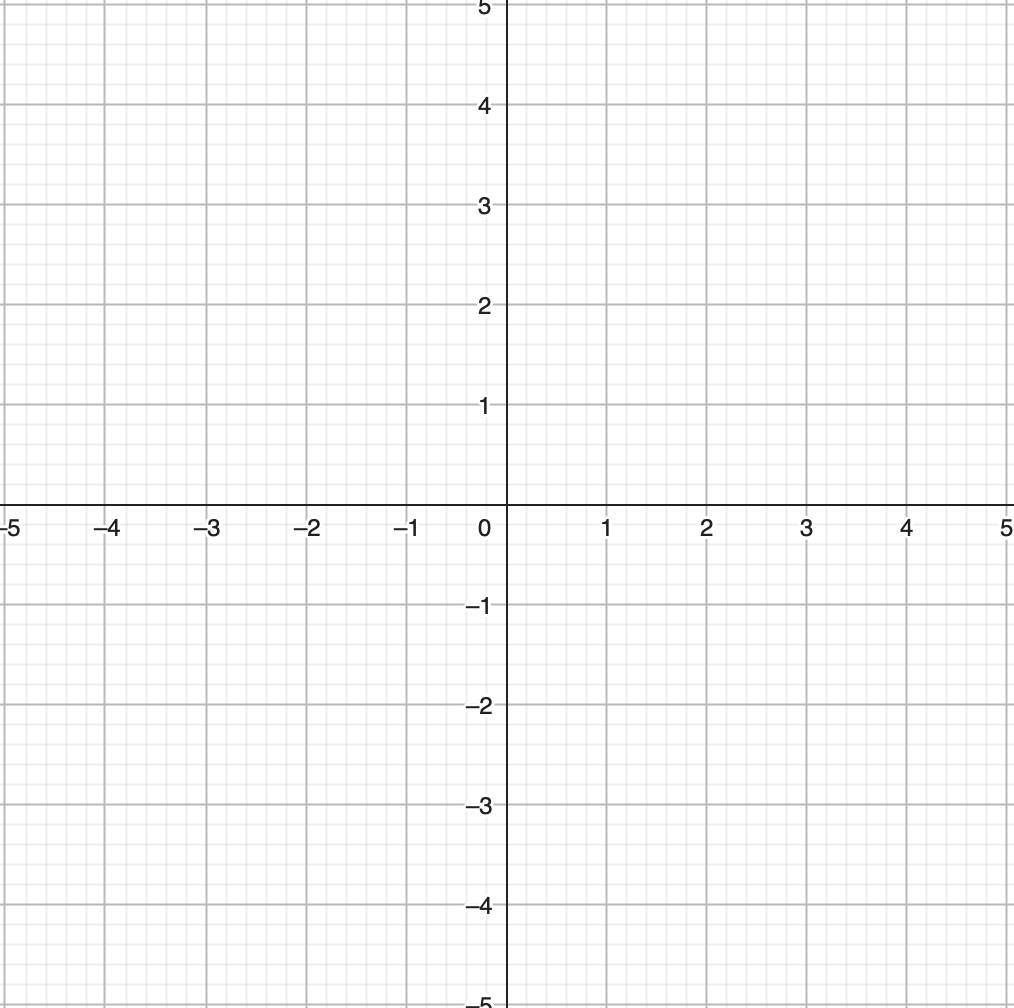
\includegraphics{images/CP-1-LT-1-grid-F23.png}} \\
\end{center}


	\item % Now make this one tabular and with complicated functions
Consider the two piecewise linear functions $r$ and $s$ given by the figure below.  Determine each of the following derivative values that involve functions that are defined in terms of $r$ and $s$.  Clearly show your work and thinking using proper notation, be sure your values are \emph{exact} in light of the given information, and write one sentence to explain your overall approach.
	
\begin{center}  
\scalebox{0.4}{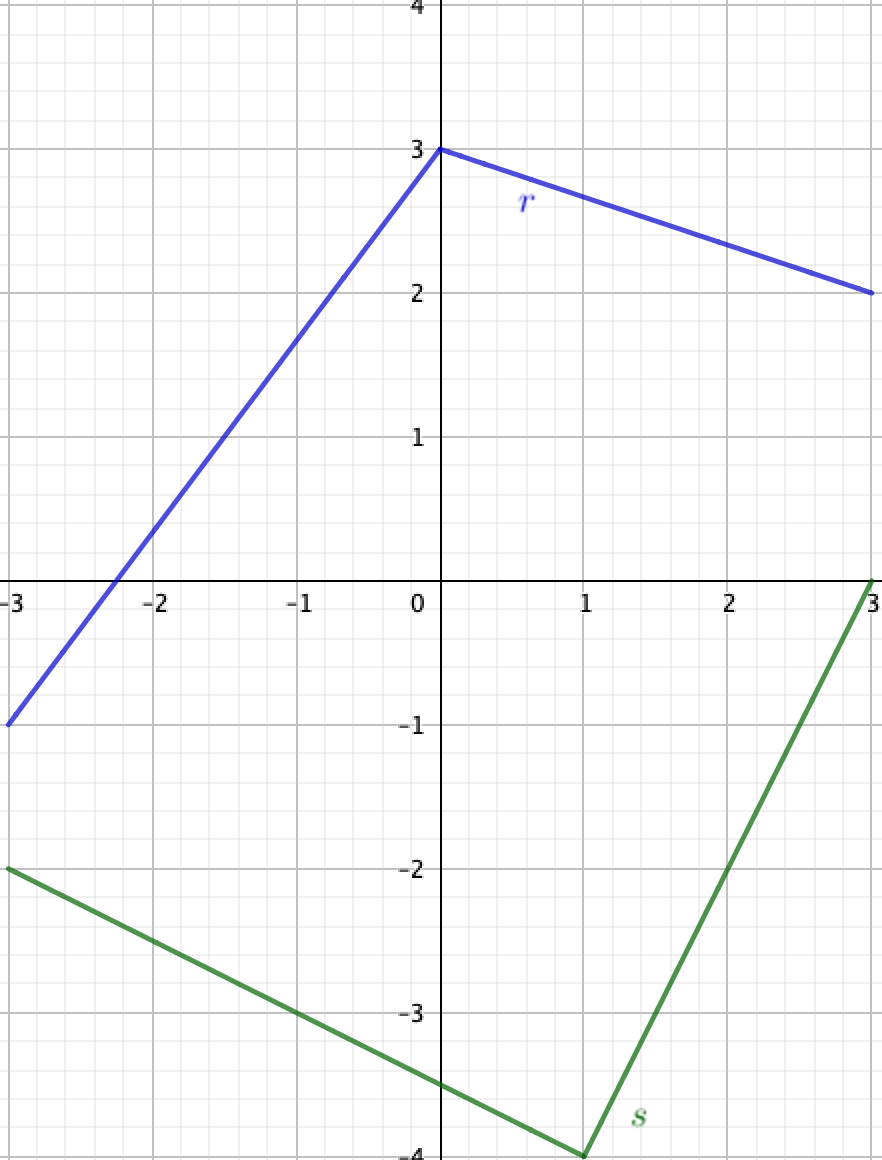
\includegraphics{images/CP7-01-3LTs.png}} \hspace{0.5in} \scalebox{0.6}{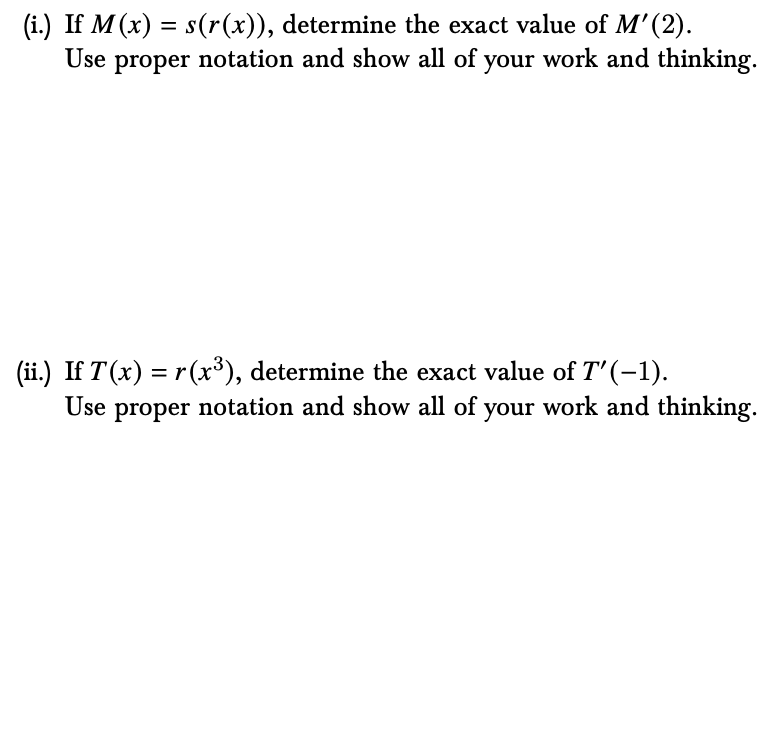
\includegraphics{images/CP3-LT1-chain.png}}
\end{center}


	
%	\be
%		\item[(i.)] If $M(x) = s(r(x))$, determine the exact value of $M'(2)$. \\  
%		Use proper notation and show all of your work and thinking.
%		\lr \tr
%		\item[(ii.)] If $T(x) = r(x^3)$, determine the exact value of $T'(-1)$. \\   
%		Use proper notation and show all of your work and thinking.
%		\lr \tr
%	\ee


%\begin{itemize}
%	\item[(i.)] $N(x) = h(x^3+2x)$.  Determine $N'(-1)$.
%	\lr
%	\item[(ii.)]  Let $R(x) = \sqrt{g(x)}$.  Determine $R'(2)$.
%	\lr
%\end{itemize}	

		\item Evaluate the following definite integral exactly using the Fundamental Theorem of Calculus.  Show your full work and thinking using proper notation.
		
		$\ds \int_{\pi/2}^{\pi} \left(\sin(x) + 2e^x - \frac{1}{x} \right) \, dx$
	\ee
	
	\vfill \hfill {\bf OVER}
	
	\pagebreak
	
	
	\item[2.]  Consider the piecewise linear function $y = f(x)$ pictured below; assume that $f(x) = 0$ for $x \le -1$ and $f(x) = 1$ for $x \ge 11$.
	
	\begin{center}
		\scalebox{0.36}{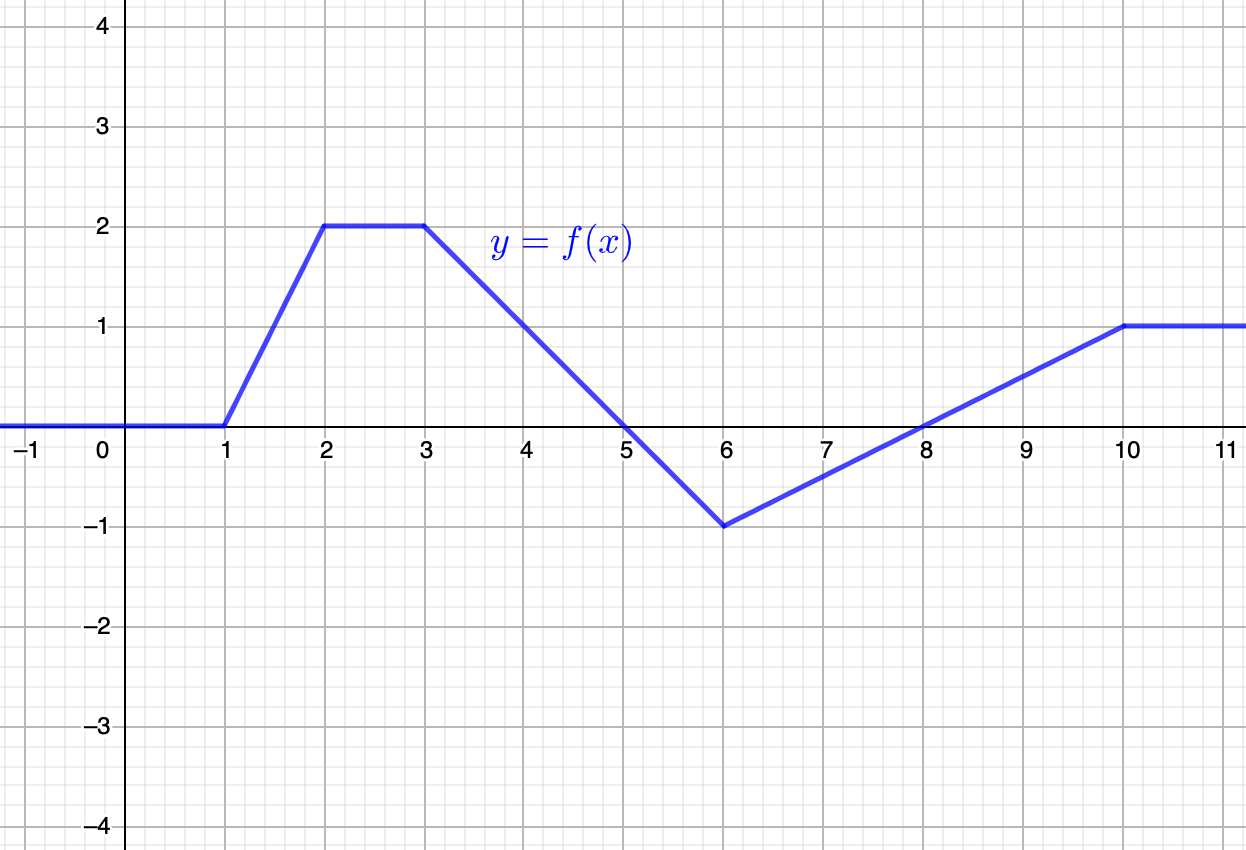
\includegraphics{images/CP-3-LT2-graph.png}} \hspace{0.25in} \scalebox{0.36}{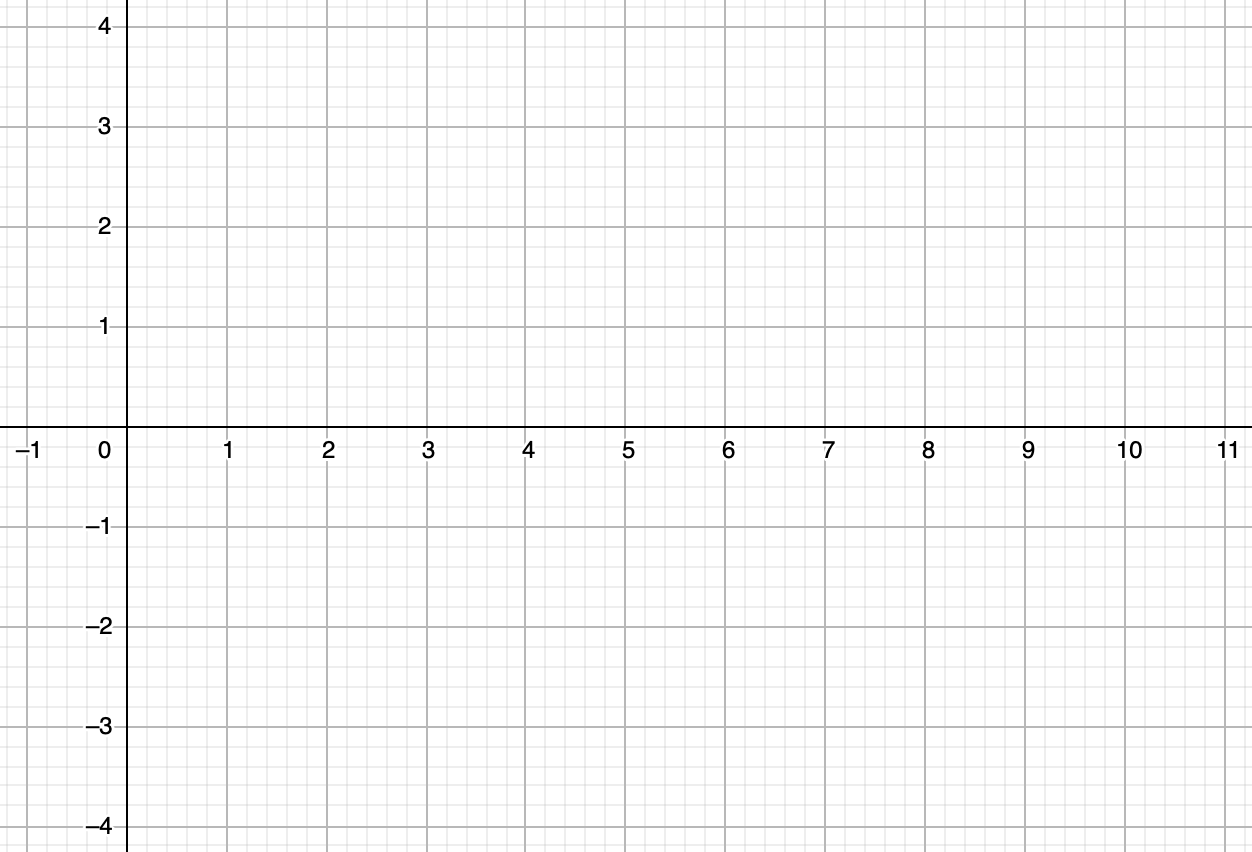
\includegraphics{images/CP-3-LT2-grid.png}} 
	\end{center}
	
	Let $F$ be an antiderivative of $f$ that satisfies $F(1) = -2$.
	
	\be
		\item On what intervals is $F$ increasing?  decreasing? neither?  why?
		
		\lr
		
		\item On what intervals is $F$ concave up?  concave down?  neither?  why?
		
		\lr
		
		\item Find the exact values of $F(2)$, $F(3)$, $F(5)$, $F(6)$, $F(8)$, and $F(10)$.  Write one sentence to explain briefly how you found these values.
		
		\mr
		
		\item On the blank grid at right, sketch an accurate, labeled graph of $y = G(x)$.
		
	\ee

\pagebreak

%{\bf LT 3}: I can apply the Second Fundamental Theorem of Calculus to find the antiderivative of a function in terms of an integral and also use the FTC to differentiate an integral function. (Section 5.2)

	\item[3.] \ 
	\be
		\item State an antiderivative $H$ of the function $\ds h(x) = \frac{4}{e^{x^2} + x^2 + 2}$ that has the property that $H(-1) = -3$.  Write one sentence to explain how you determined your formula.
		
		\lr \tr
		
		\item Suppose that $y = g(x)$ is the piecewise function given by the graph below, and let $G(x) = \int_3^x g(t) \, dt$.
		
	\begin{center}
		\scalebox{0.5}{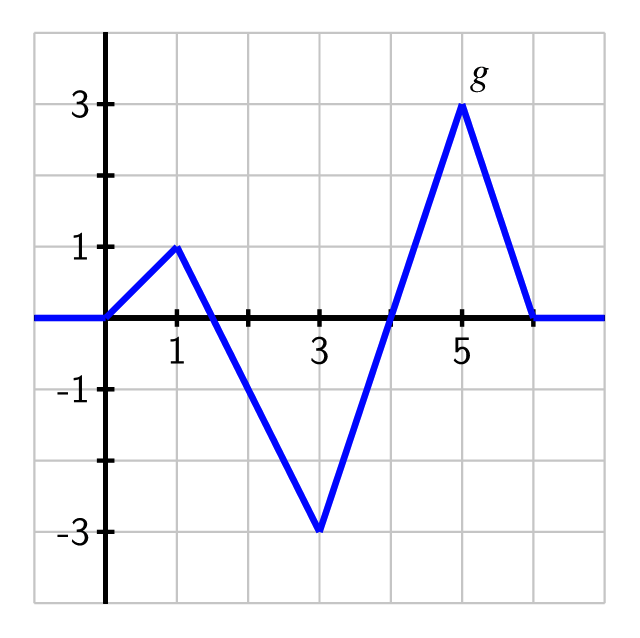
\includegraphics{images/CP-3-LT3-graph.png}} 
	\end{center}
	
		\be
			\item Determine $G'(5)$.  Write briefly to explain how you found its value.
			
			\lr
			
			\item For what $x$-value(s) is $G'(x)$ an increasing function?  Why?
		\ee
	\ee
		

\pagebreak

\item[4.] Evaluate each of the following integrals either using $u$-substitution or integration by parts.  For each, \emph{(i) clearly state your substitution/method including any new variables you use, (ii) show all of your work, and (iii) write one sentence that explains what motivated your choice of method and substitution}.  Your process is even more important than your answer in each.

			\be
				\item $\ds \int x^3 \cos(5x^4) \, dx$
			
				\mr \tr
			
				\item $\ds \int x \sin(5x) \, dx$
			
				\mr \tr
				
				\item $\ds \int \sin(x) e^{\cos(x)} \, dx$
			\ee
	
%		\item Consider an integral of the form
%		$$\int 4x \sin(f(x)) \, dx$$

%			\be
%				\item	Give an example of a function you could choose for $f(x)$ that would allow you to evaluate the integral $\int 4x \sin(f(x)) \, dx$ using $u$-substitution.   State your function $f(x)$ clearly and state the full $u$-substitution you'd use, but {\bf don't} actually evaluate the integral.  \emph{Write a sentence to explain your thinking.}
				
%				\lr
				
%				\item Give an example of a function you could choose for $f(x)$ that would allow you to evaluate the integral $\int 4x \sin(f(x)) \, dx$ using integration by parts.   State your function $f(x)$ clearly and state the full substitution you'd use (that is, state $u$, $du$, $dv$ and $v$, but {\bf don't} actually evaluate the integral.  \emph{Write a sentence to explain your thinking.}
%			\ee
%	\ee
\end{enumerate}




\end{document}

